\section{Final Design}

LARRE's leg segments are constructed from 6061 aluminum alloy concentric sliding pipes with clamps allowing the joints' to be adjusted for each person. This material is lightweight and easy to manufacture. The axles of the joints were constructed of steel to handle the expected stress. Safety is a significant concern; careful attention was given to the manufacturing process to minimize the sharp edges since it is attached to a human-machine interface system. Safety is essential for people with SCI who have minimal sensory abilities and would not feel an injury.  LARRE is attached to a person through the upper body and waist straps. Custom-made 3D printed strap carriages are placed on the thigh and shank segment and connect the person to the exoskeleton's legs. \autoref{fig:LARRE} shows the final model of LARRE.     


\begin{figure}
    \centering
    \includegraphics[scale=0.08]{images/mech_design/exo_side2.png}
    \caption{The LARRE exoskeleton being worn}
    \label{fig:LARRE}
\end{figure}


The dynamic properties of LARRE are essential for building the controller. The dynamics of LARRE were calculated using SolidWorks. The properties account for the material properties of the components as well as the geometry. \autoref{tab:LARREMASS} summarizes the dynamic properties of LARRE. The exoskeleton has defined joint limits to allow for biological motion, summarized in \autoref{tab:jointlimits}.

\begin{table}[h!]
    \centering
    \begin{tabular}{|c c c c c|}  
         \hline 
          \multicolumn{5}{|c|}{Exoskeleton Segment Parameters} \\
         \hline
         Link & Mass (kg) & $CoM_x$ & $CoM_y$ & $CoM_z$ \\
         \hline \hline
         Hip & 2.3677 & 0.000011338 & 0.093937 &  -0.12619 \\
         Thigh & 2.1138 & 0.0034745   & 0.097979 &  0.1712 \\
         Shank & 1.2804  &   0.002761 & 0.097563   & 0.15581\\
         Foot & 0.85523 & 0.14092 & 0.2267 &  -0.31138  \\
         \hline
    \end{tabular}    
    \caption[Dynamic Properties of the LARRE]{Mass Properties of the LARRE}
    \label{tab:LARREMASS}
\end{table}


\begin{table}[h!]
\begin{centering}
    \begin{tabular}{ |p{1cm} p{2cm} p{2cm} |  }
        \hline 
        \multicolumn{3}{|c|}{LARRE Joints Limits} \\
        \hline 
        Joint & Flexion & Extension \\
        \hline \hline
        Hip   & $-60^{\circ}$   & $30^{\circ}$  \\
        Knee &   $-110^{\circ}$  & $0$   \\
        Ankle & $-20^{\circ}$ & $20^{\circ}$  \\
        \hline
    \end{tabular}
    \caption[LARRE Joint Limits]{Joint limits}    \centering
    \label{tab:jointlimits}
\end{centering}
\end{table}


A single patient study was conducted to measure the kinematics and dynamics of a gait while wearing LARRE. This study was not designed to measure the ability of the exoskeleton to induce movement but merely to observe the motion of the exoskeleton. The Vicon setup described in \autoref{sec:setup} was used with the custom marker layout shown in \autoref{fig:larremarker}. Additional markers were added to the plug-in gait model. \autoref{tab:exomarkerlayout} details the rigid bodies used and their location (see \autoref{fig:markers} for definition of the marker layout). The additional markers were added to ensure that there was no marker occlusion during the trial. 


\begin{table}[h!]
    \begin{centering}
            \begin{tabular}{||c  c ||} 
         \hline
            Plate Name & Plate \#  \\ [0.5ex] 
            \hline\hline
            LTHIGH	& 11 \\
            LSHANK &	19\\
            LFOOT &	9 \\
            LTHIGH FRONT &	7\\
            LTHIGH BACK &	15\\
            LSHANK FRONT &	4\\
            LSHANK BACK &	14\\
            RTHIGH SIDE &	5\\
            RSHANK SIDE &	17\\
            RFOOT &	10\\
            RTHIGH FRONT &	20\\
            RTHIGH BACK &	16\\
            RSHANK FRONT &	1\\
            RSHANK BACK &	3\\
            BACK &	2\\ [1ex] 
         \hline
        \end{tabular}
        \caption[Exoskeleton Rigid Body Numbers]{Rigid Body Numbers}
        \label{tab:exomarkerlayout}
    \end{centering}
\end{table}

The joint kinematics are shown in \autoref{fig:exojointkin}. Only a single demonstration is shown; however, multiple demonstrations were recorded. Similarly, data were recorded for both legs, but just the right leg is shown. The heel strikes and toe-offs are pointed out in the graphs. These points are calculated using the Vicon plug-in gait tools. All of the data presented were extracted and analyzed using the tools discussed in \autoref{chap:software}. In this study, three steps were taken across the mocap floor. The first step was slightly off since it started with feet together; however, steps two and three aligned with the expected motion. The gait cycles are presented over the collected frames; the Vicon records at $100fps$, so the presented trial is approximately $14.04s$. LARRE was able to move through the desired joint range for a gait cycle. Similarly, with the moments shown in \autoref{fig:larregaitmoments}, the first step did not contain relevant data since the moments can only be calculated when the force plates embedded on the floor are stepped on. The moments are presented in $\frac{Nm}{Kg}$ which allows for the torque to be abstracted and calculated for the different masses. 








\begin{figure}[h!]
    \begin{subfigure}{0.5\textwidth}
        \centering
        \captionsetup{justification=centering}
        \centerline{
        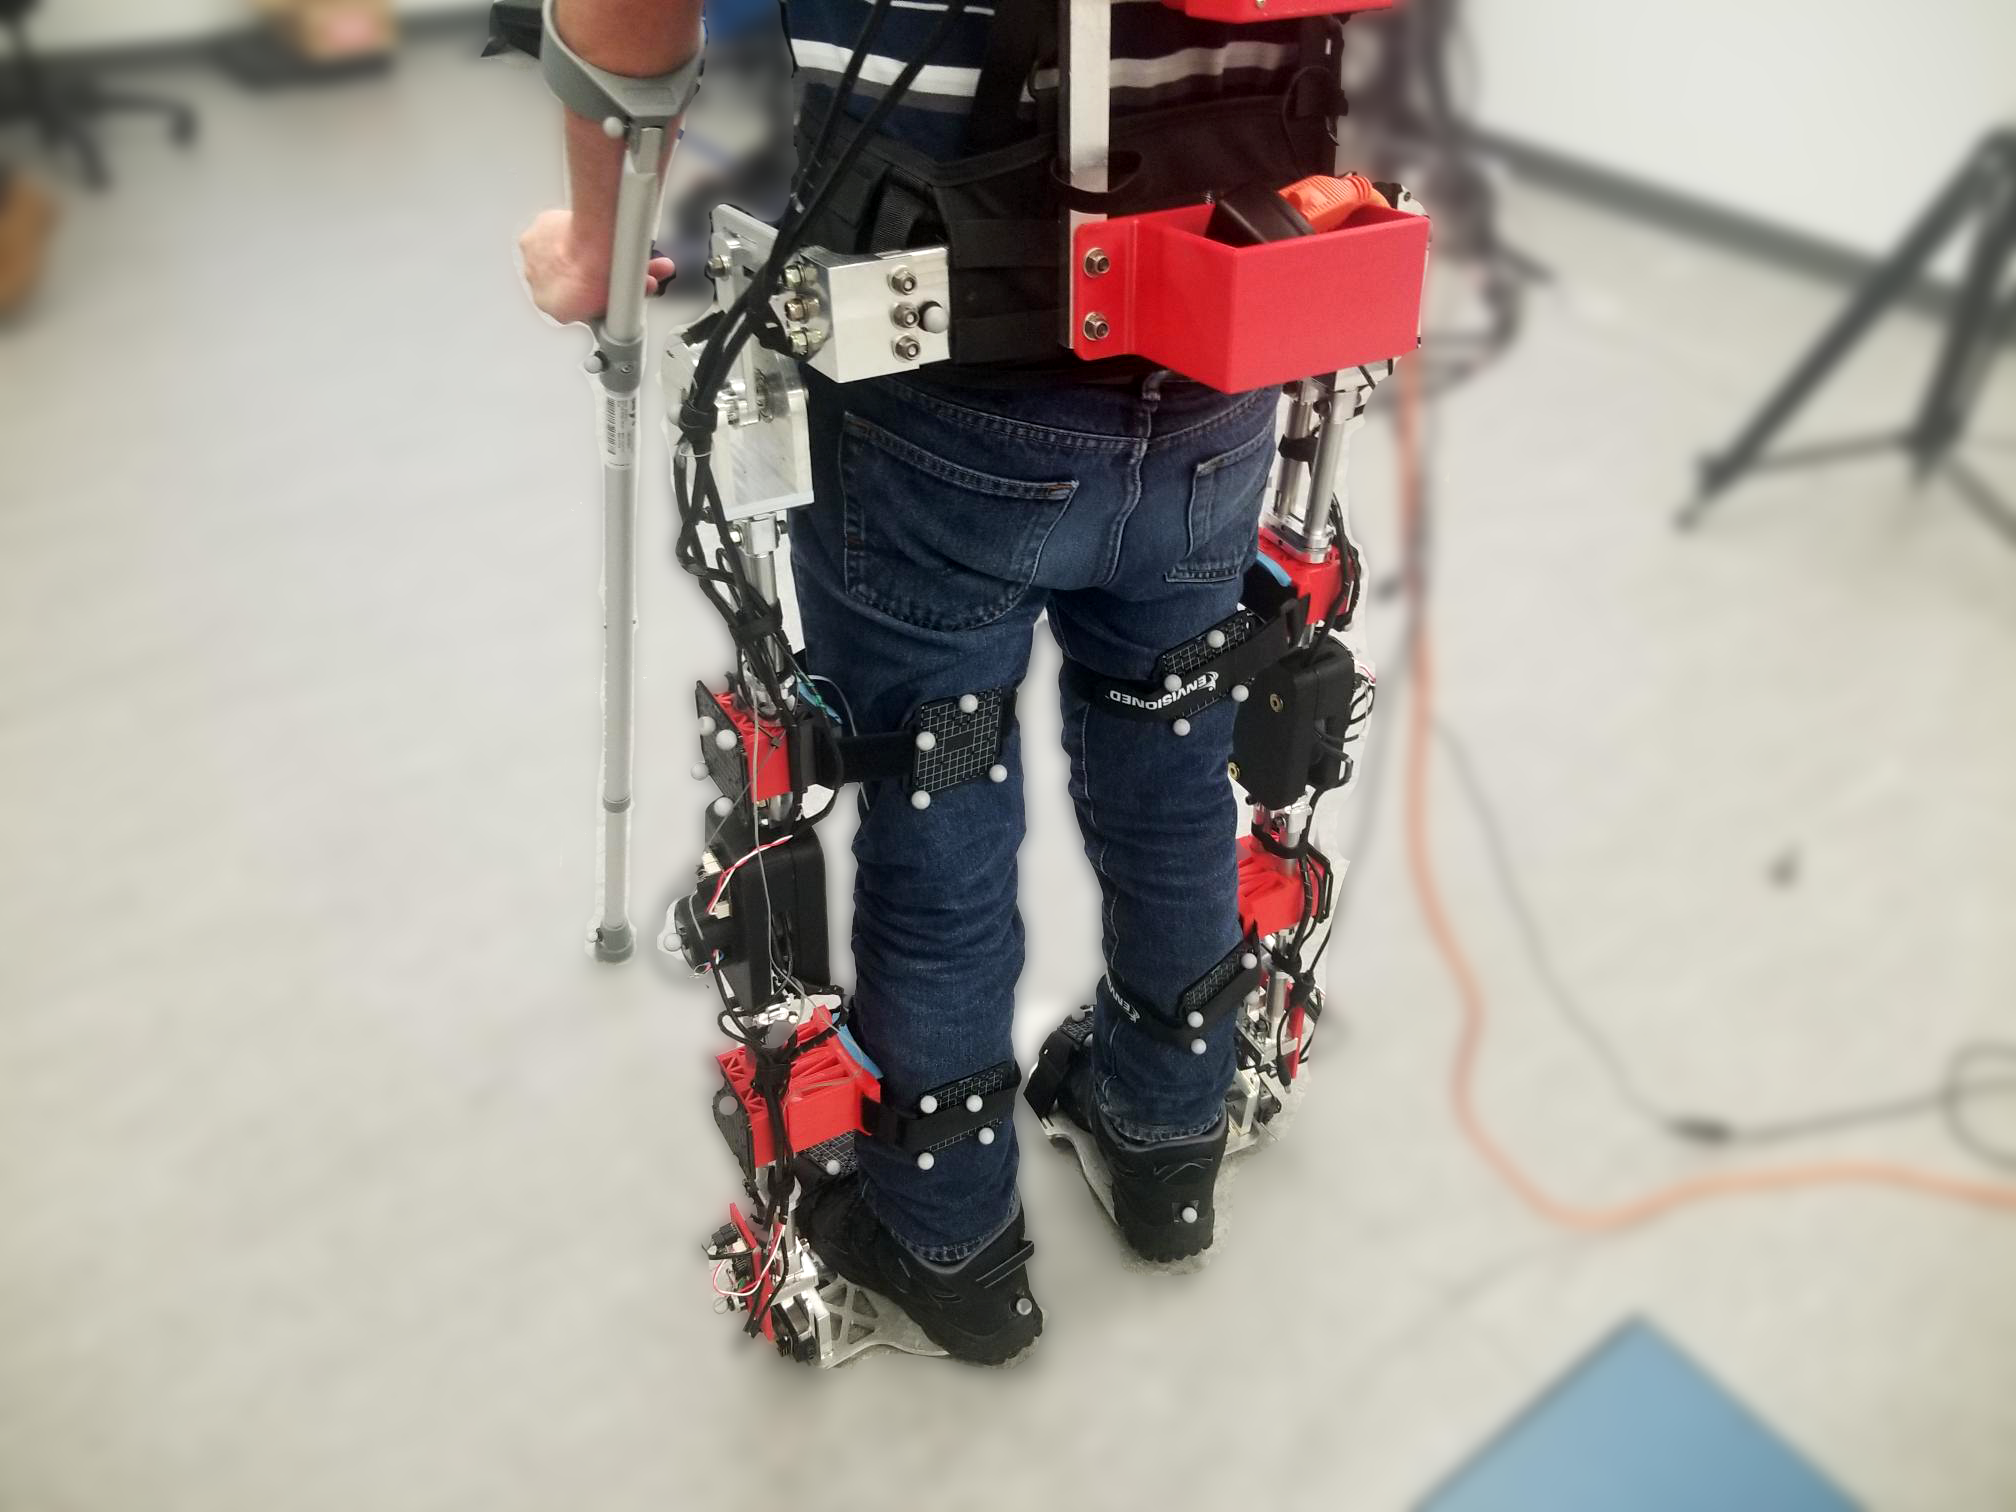
\includegraphics[scale=0.1, frame]{images/mech_design/exo_markers_back.png}}
        \caption[LARRE marker set back/side]{LARRE marker set back/side}
        \label{fig:larremarkerside}
    \end{subfigure}
    \begin{subfigure}{0.5\textwidth}
        \centering
        \captionsetup{justification=centering}
        \centerline{
        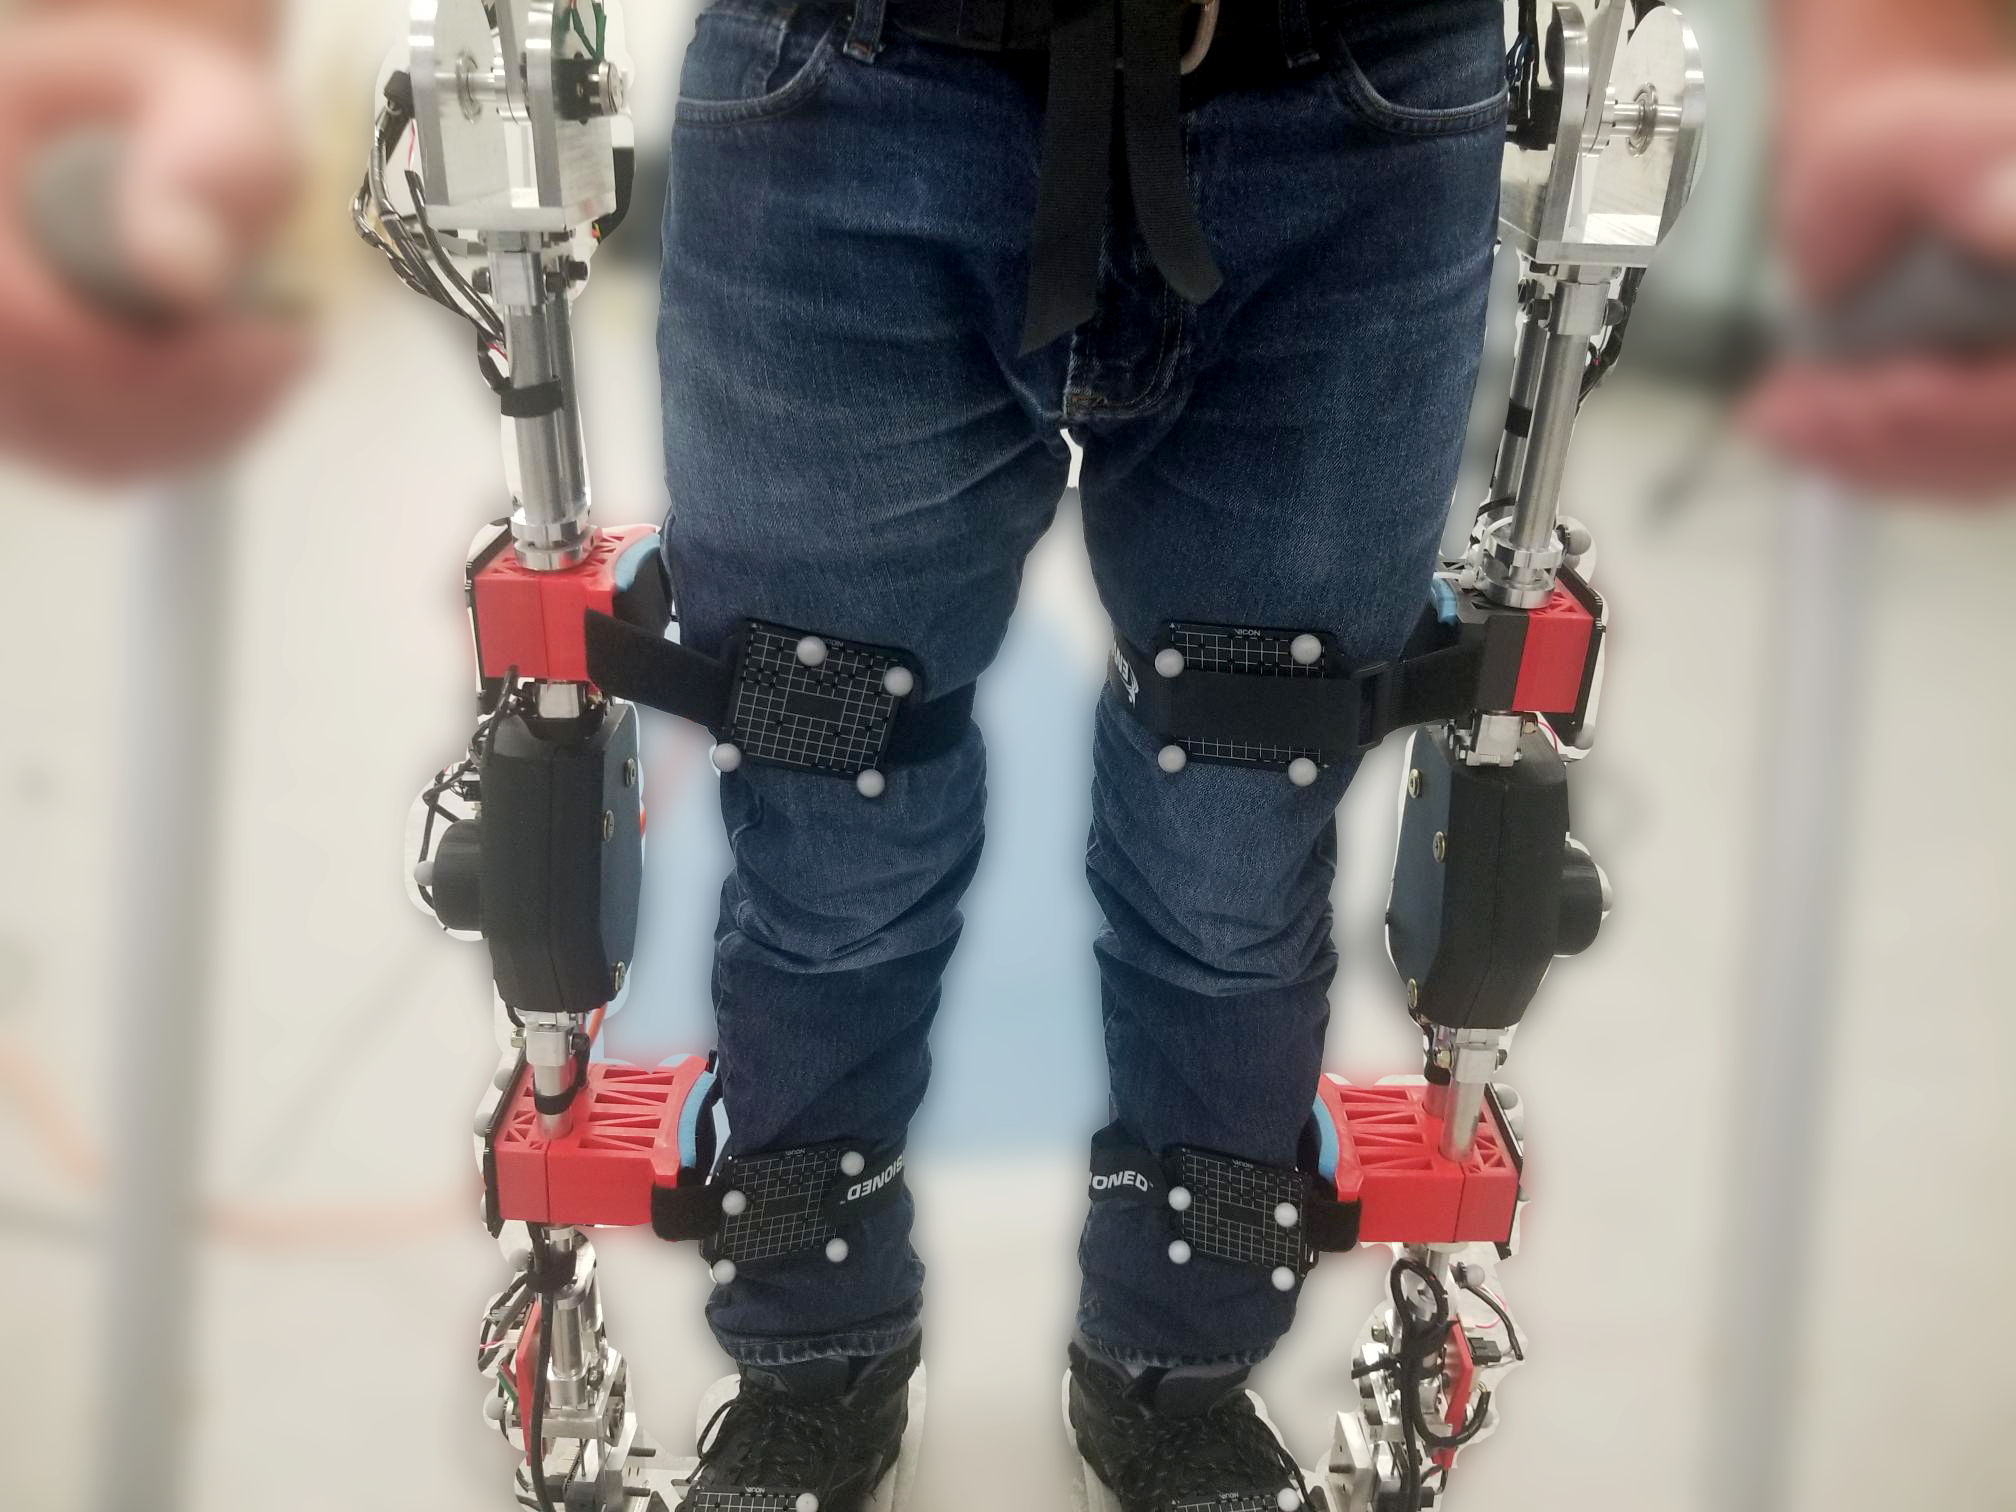
\includegraphics[scale=0.1, frame]{images/mech_design/exo_markers_front.png}}
        \caption[LARRE marker set front]{LARRE marker set front}
        \label{fig:larremarkerfront}
    \end{subfigure}    
    \caption{Marker set for LARRE}
    \label{fig:larremarker}
\end{figure}



\begin{figure}
    \begin{subfigure}{\textwidth}
        \centering
        \captionsetup{justification=centering}
        \centerline{
        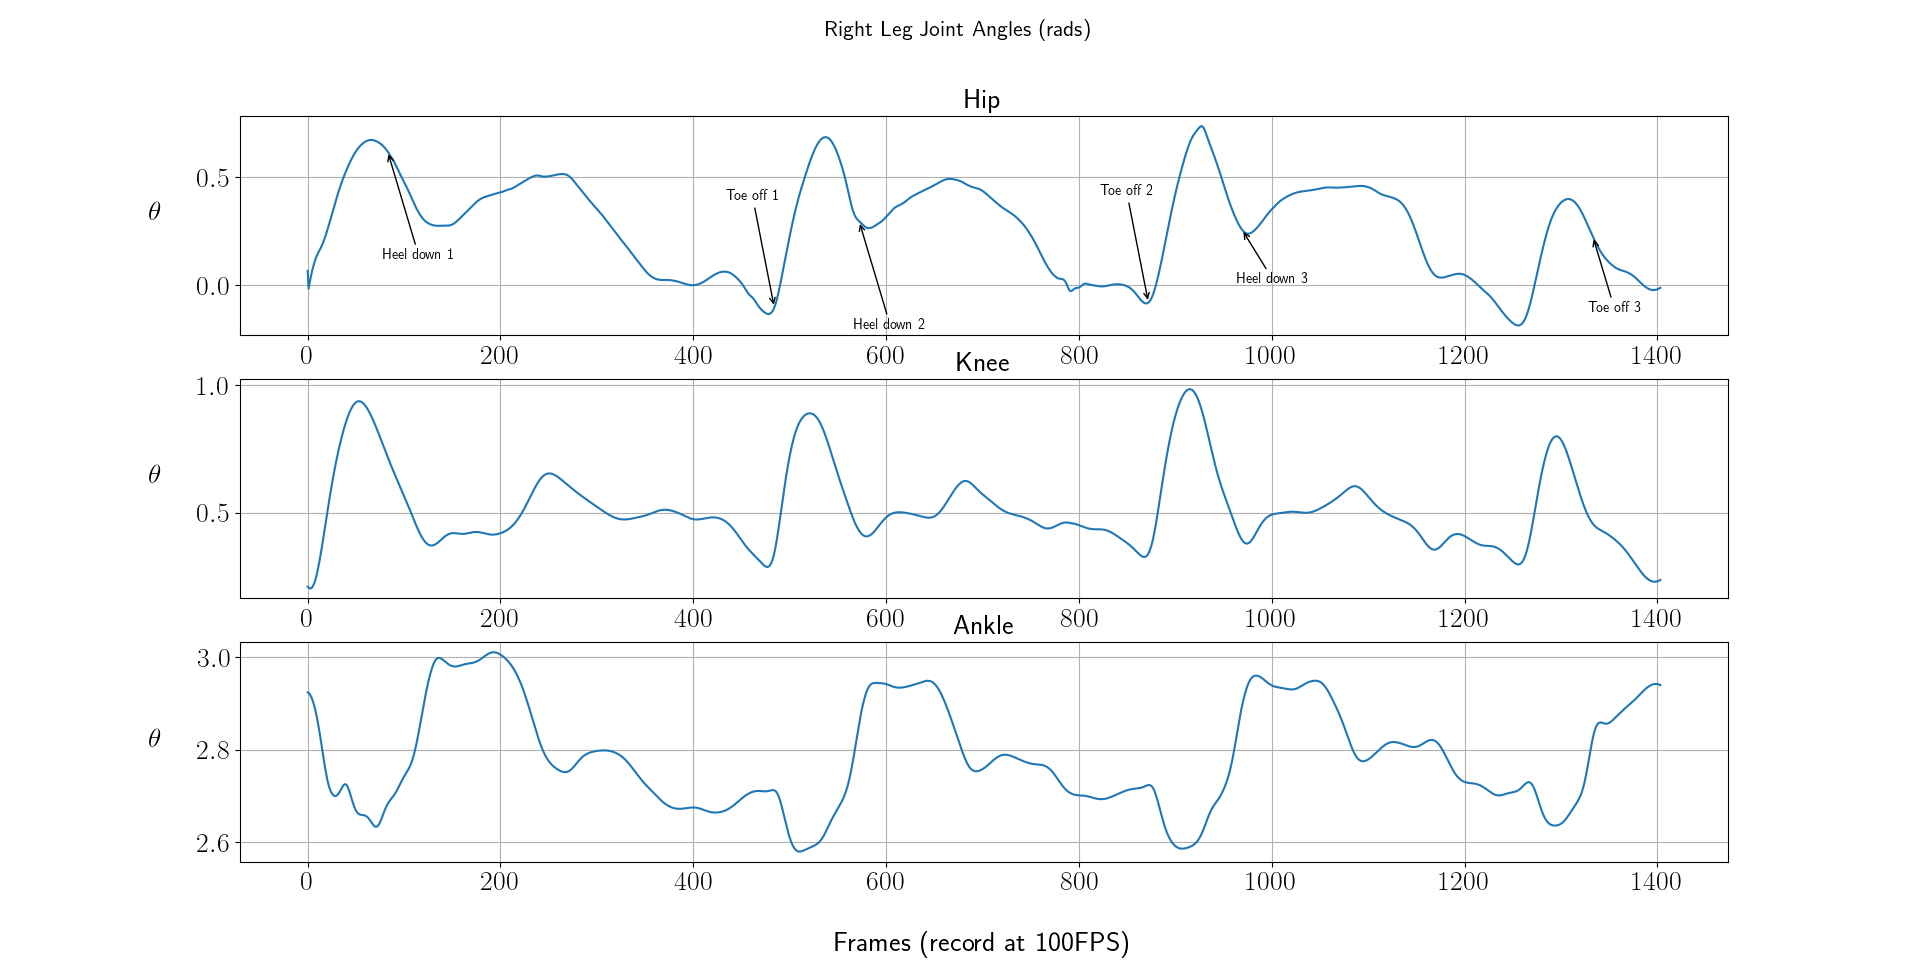
\includegraphics[width=\textwidth, frame]{images/mech_design/exo_joint_angles.png}}
        \caption[LARRE gait cycle angles]{Gait cycle angles of the LARRE}
        \label{fig:larregaitangles}
    \end{subfigure}
    \begin{subfigure}{\textwidth}
        \centering
        \captionsetup{justification=centering}
        \centerline{
        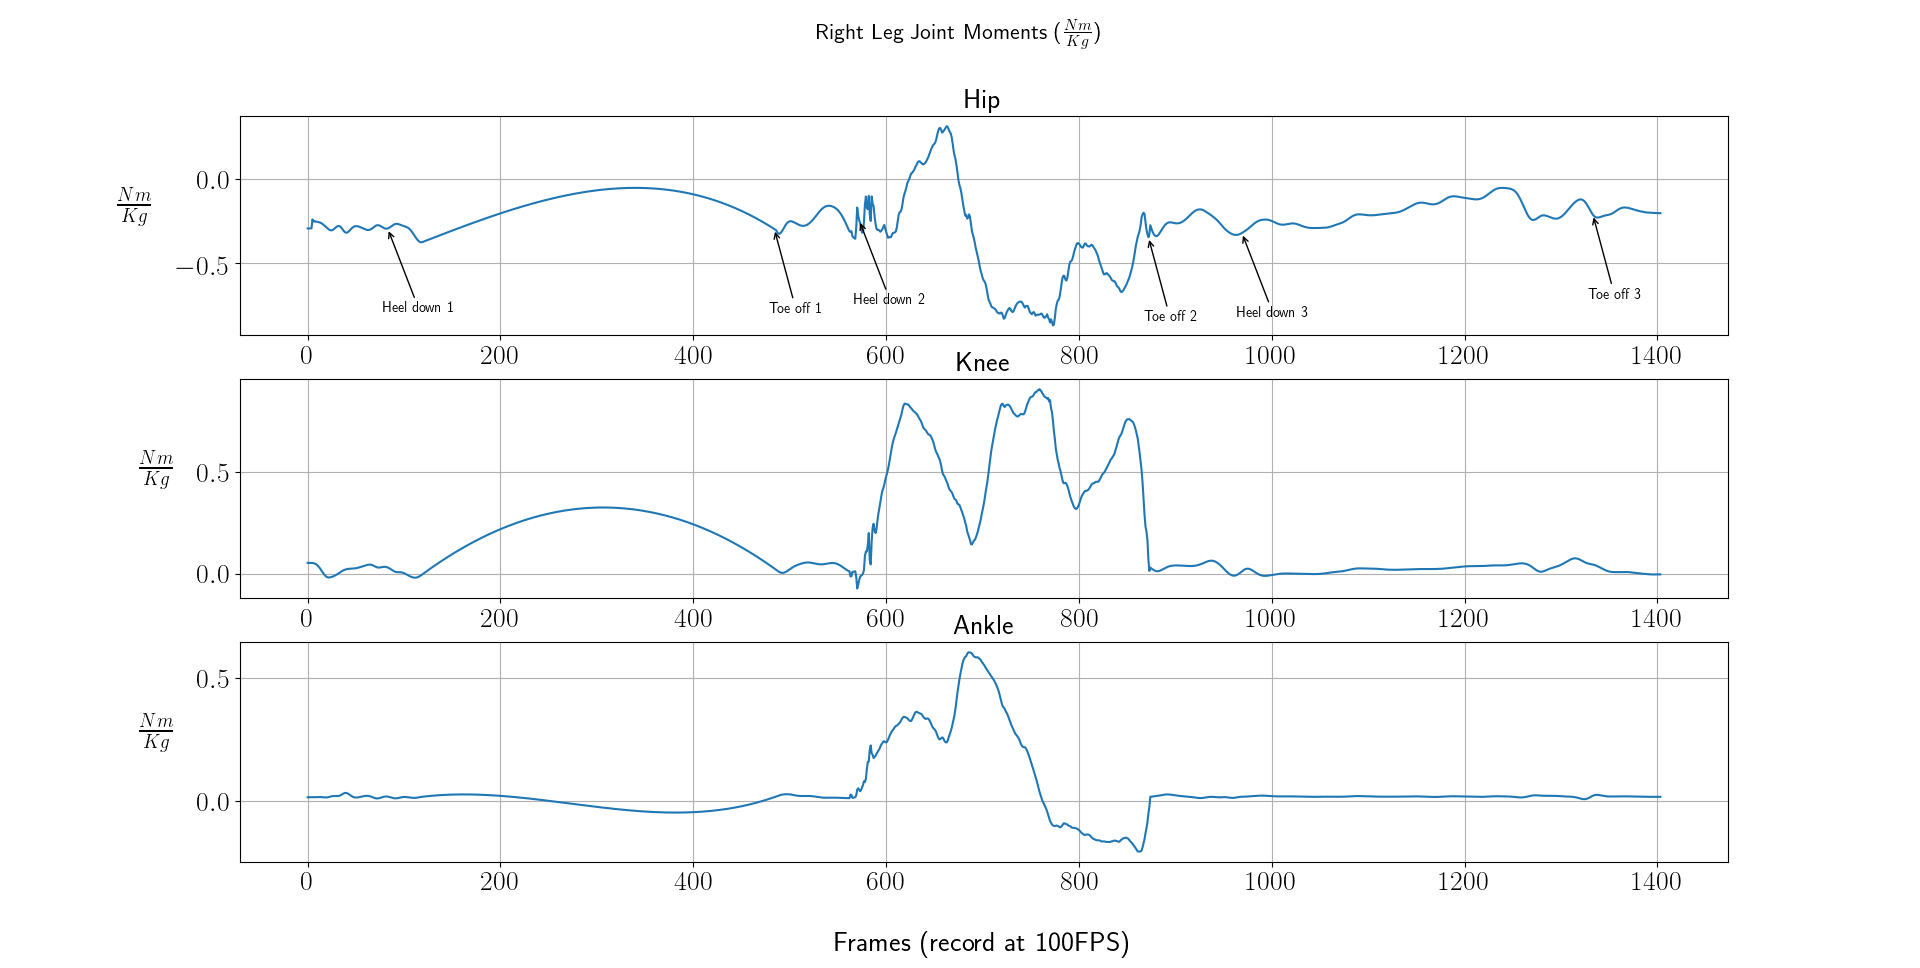
\includegraphics[width=\textwidth, frame]{images/mech_design/exo_joint_moments.png}}
        \caption[LARRE gait cycle moments]{Gait cycle moments of the LARRE}
        \label{fig:larregaitmoments}
    \end{subfigure}
    \caption{Gait cycles kinematics for LARRE}
    \label{fig:exojointkin}
\end{figure}




\autoref{fig:positioncomparison} compares the position of the LARRE to the that human. The positional difference has a maximum displacement between $10mm-20mm$. \autoref{fig:markerpositiondiagram} shows a diagram of the marker position on the thigh segment and LARRE with a simplified model that illustrates the calculation.  This difference was measured be using the front and back rigid body plates on the legs and on the side of the exoskeleton. The centroid of the front/back markers was taken as the location of that body segment. The mean position was removed to only show the average change in position over the course of the trial.  

\begin{figure}[h!]

    \begin{subfigure}{\textwidth}
        \centering
        \captionsetup{justification=centering}
        \centerline{
        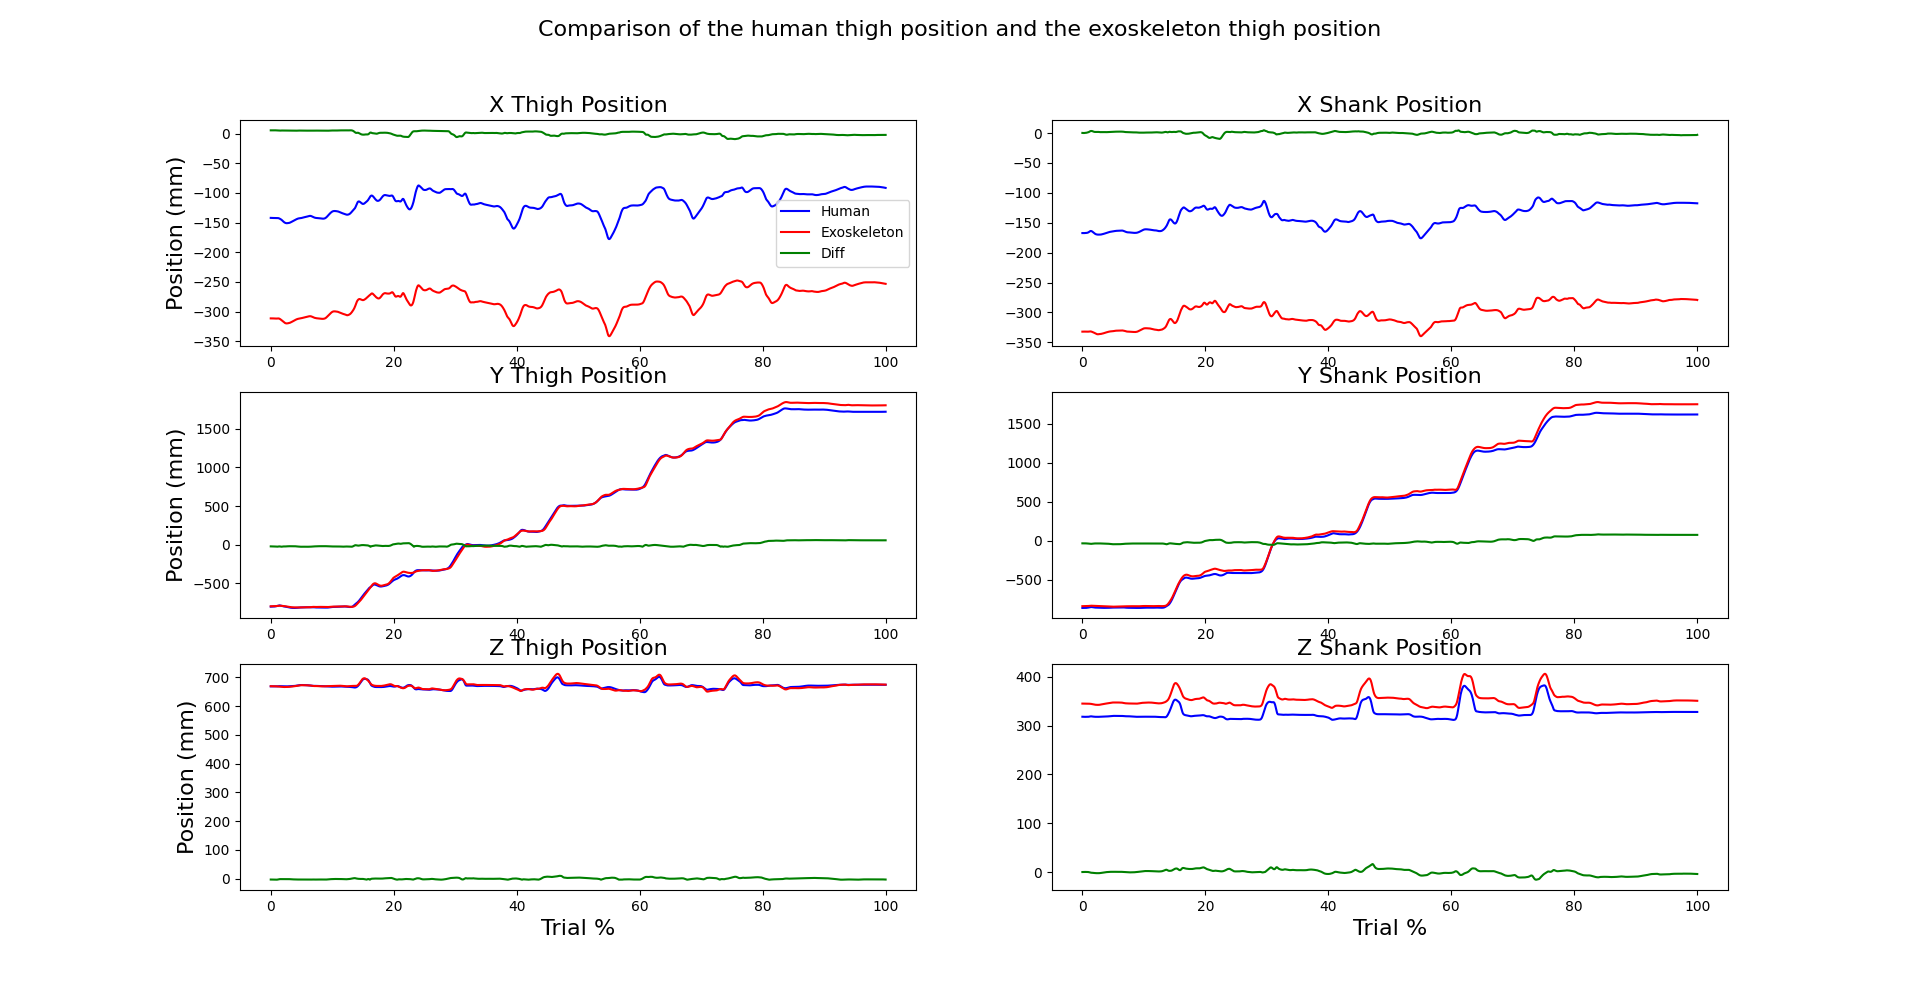
\includegraphics[width=\textwidth, frame]{images/mech_design/position_comparison.png}}
        \caption[Comparison of Difference of Human and LARRE Position]{Comparison of the human position vs. LARRE position}
        \label{fig:positioncomparison}
    \end{subfigure}
        \begin{subfigure}{\textwidth}
        \centering
        \captionsetup{justification=centering}
        \centerline{
        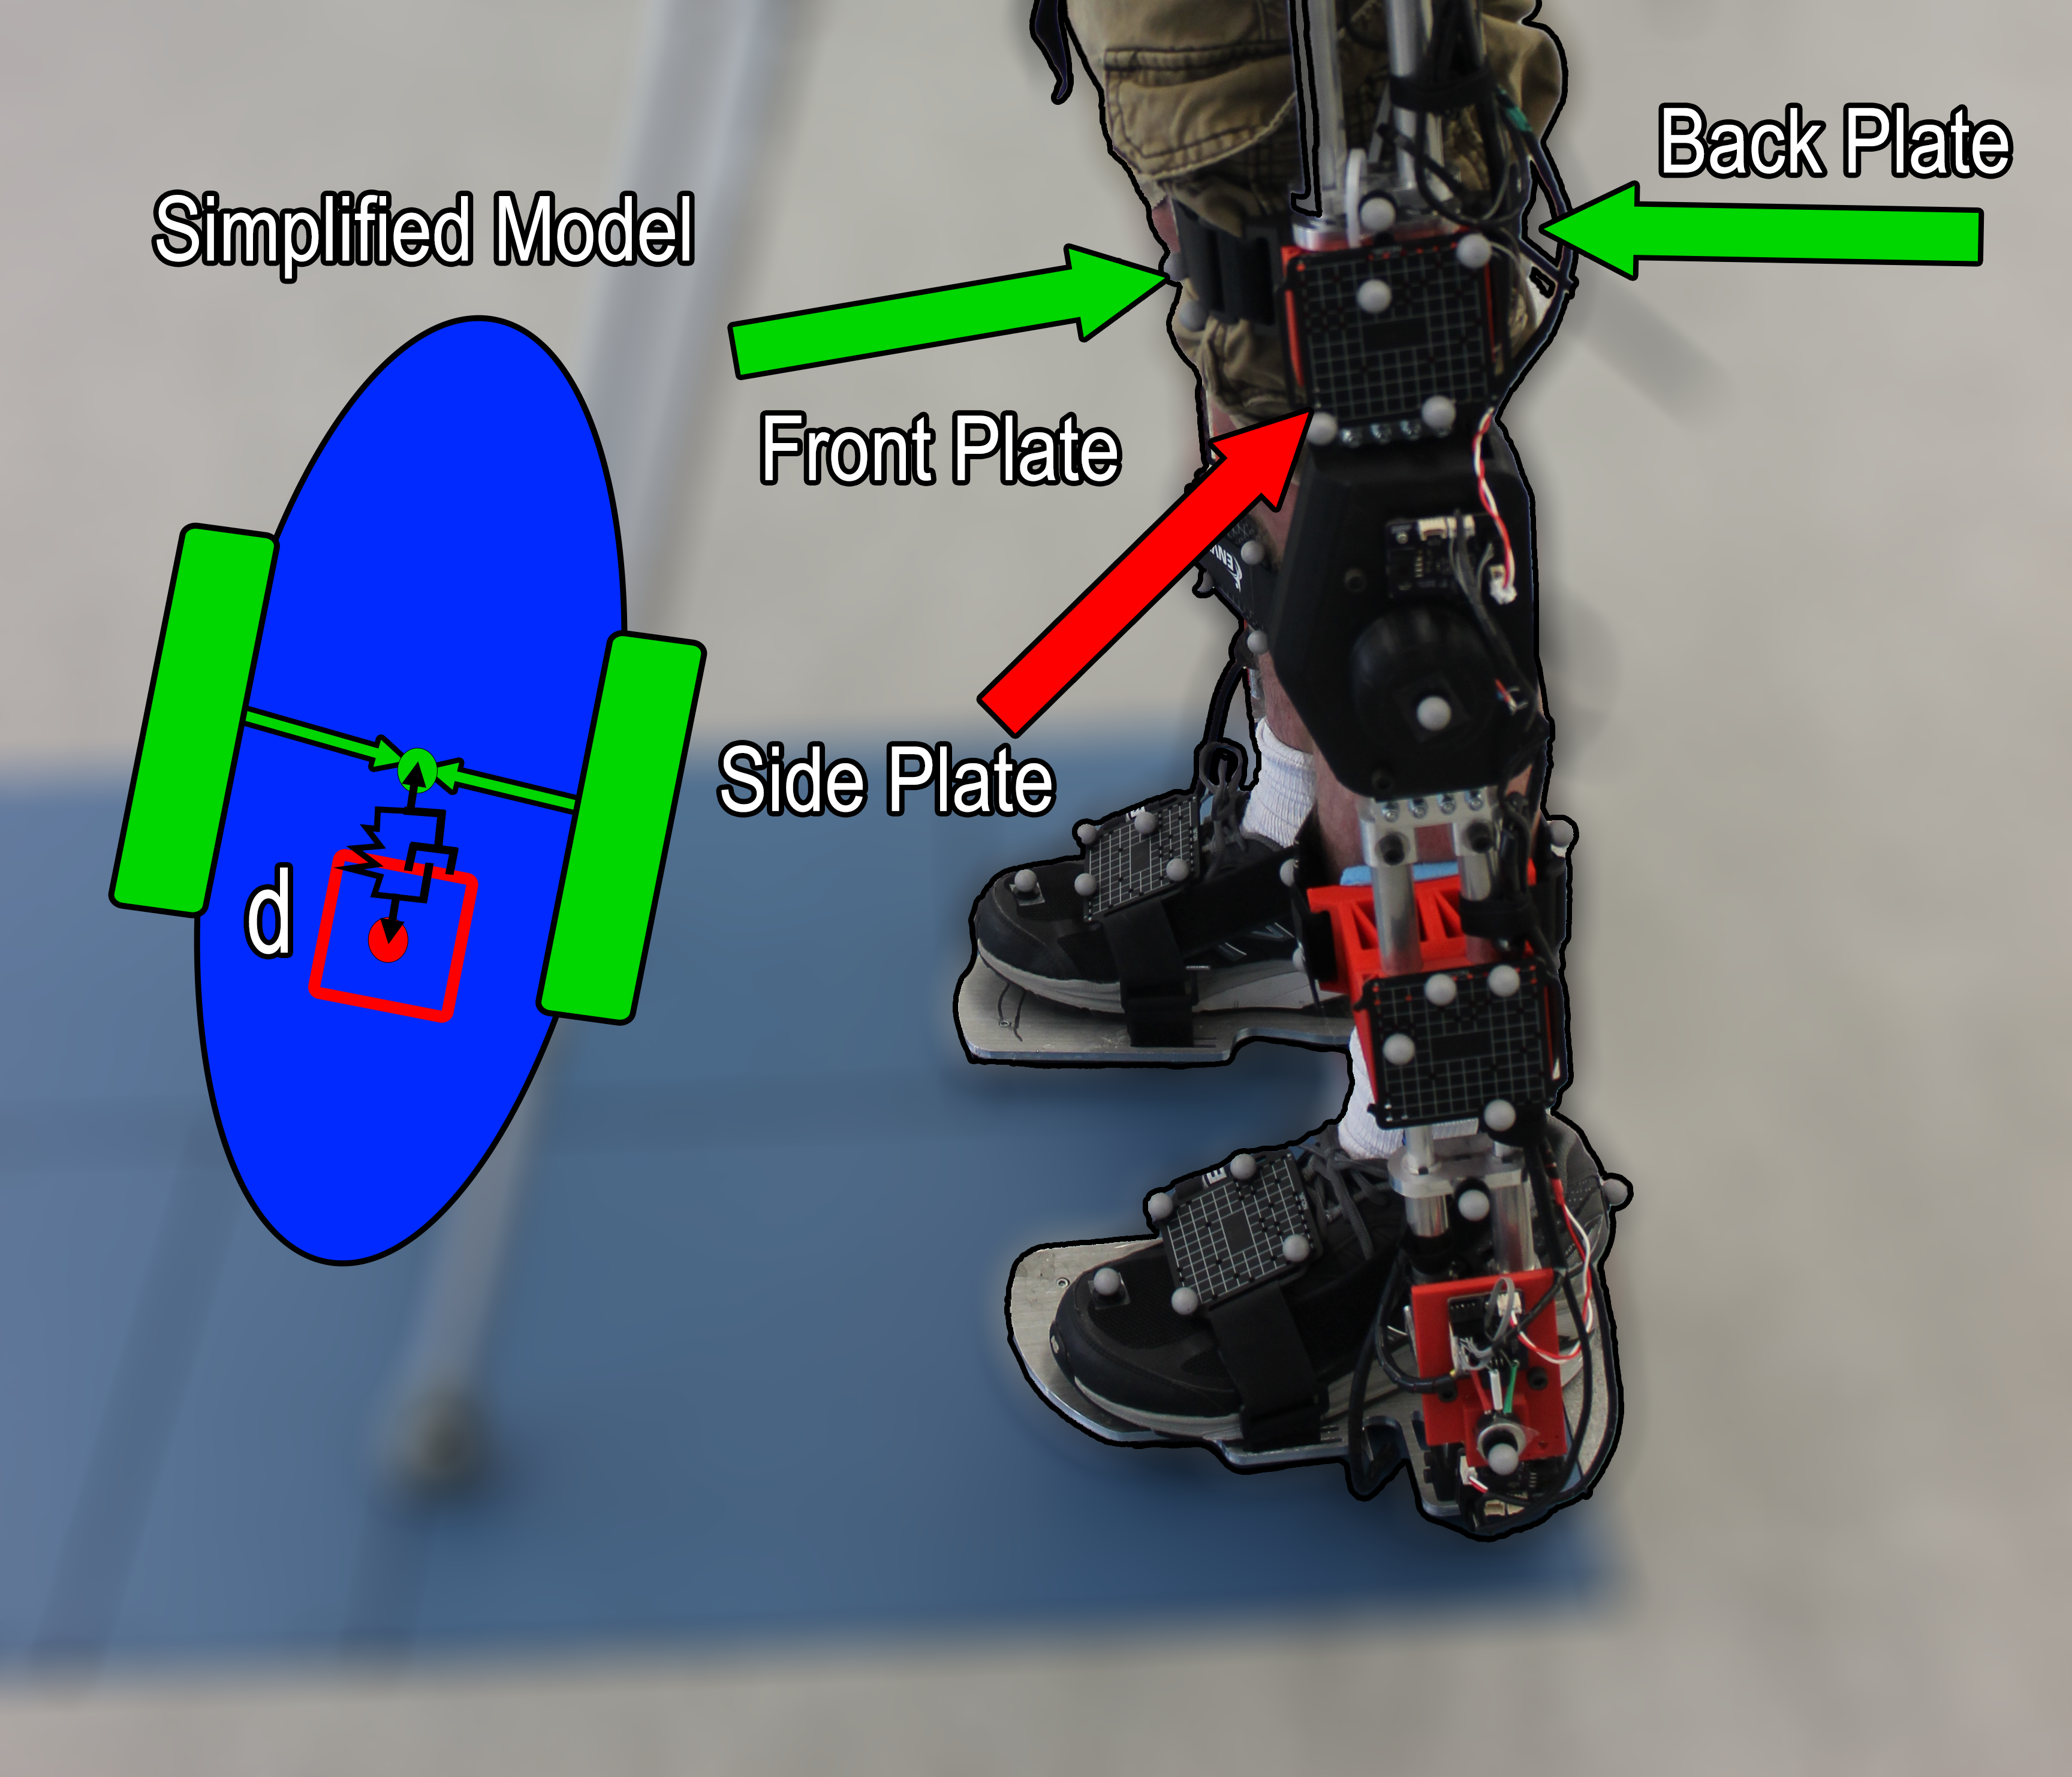
\includegraphics[width=0.5\textwidth, frame]{images/mech_design/side_marker_positioning.png}}
        \caption[Diagram of Marker Segment Measurement]{Diagram of Marker Segment Measurement}
        \label{fig:markerpositiondiagram}
    \end{subfigure}
    \caption[Comparison of LARRE and human positions]{Comparison of the positional difference of LARRE and the human.}
    \label{fig:exohumanmarkercompare}
\end{figure}


The electrical control system for LARRE is currently under development. The control board was developed by Micheal Conrad. The control board consists of a  Xilinx Zynq 7000 \footnote{https://www.xilinx.com/products/silicon-devices/soc/zynq-7000.html}  field-programmable gate arrays (FPGAs) as the primary controller for the exoskeleton. This allows for high speed communication with the motors and sensors. The control board is shown in[insert control board figure].

Additionally, custom PCB with integrated inertial measurement unit (IMU) and potentiometer connectors are placed on each of the leg segments (thigh, shank, and foot). The PCM is shown in \autoref{fig:imu_circut} Cables run down from the main control board the leg and snap into each of the IMU boards. This allows for the collection of all the sensor information.  

\begin{figure}
    \centering
    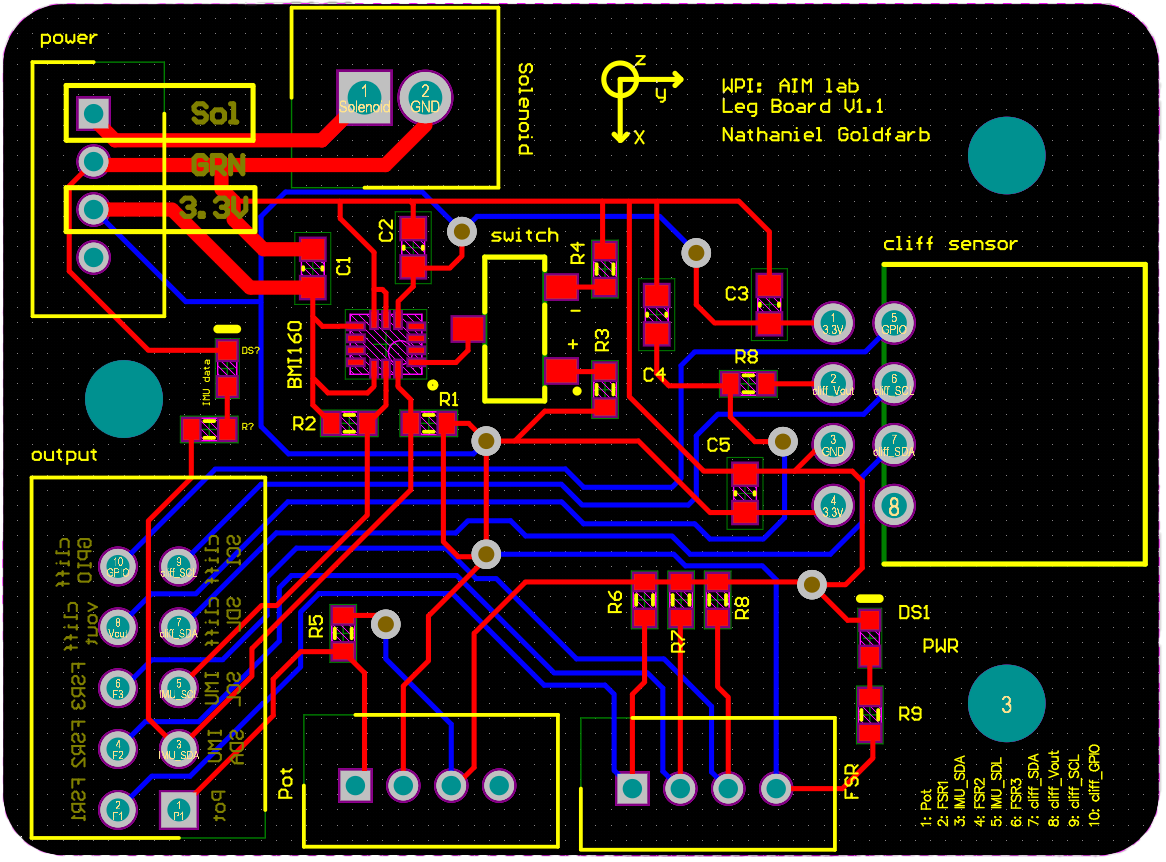
\includegraphics[scale=0.18]{images/mech_design/IMU_circut_edit.png}
    \caption{IMU circuit diagram}
    \label{fig:imu_circut}
\end{figure}

% \begin{table}[h!]
% \begin{centering}
%     \begin{tabular}{ |p{1cm} p{2cm} p{2cm} p{2cm}|  }
%         \hline 
%         \multicolumn{4}{|c|}{LARRE Joints Limits} \\
%         \hline 
%         Joint & Flexion & Extension & Torque \\
%         \hline \hline
%         Hip   & $-60^{\circ}$   & $30^{\circ}$ &  60N \\
%         Knee &   $-110^{\circ}$  & $0$  & 50N \\
%         Ankle & $-20^{\circ}$ & $20^{\circ}$ &  - \\
%         \hline
%     \end{tabular}
%     \caption[LARRE Joint Limits]{Joint limits}    \centering
%     \label{tab:biomech}
% \end{centering}
% \end{table}